\documentclass[10pt]{article}
\usepackage[margin=0.5in]{geometry}
\usepackage{hyperref}
\usepackage{xcolor}
\usepackage{lmodern}
\usepackage{microtype}
\usepackage{tikz}
\usetikzlibrary{arrows.meta,positioning,shapes.geometric,fit}

\hypersetup{colorlinks=true, linkcolor=blue, urlcolor=blue, citecolor=blue}

\makeatletter
\renewcommand{\section}{\@startsection{section}{1}{0pt}{0.4ex plus 0.1ex}{0.15ex}{\normalfont\bfseries}}
\makeatother

\setlength{\parskip}{0.15em}
\setlength{\parindent}{0em}
\pagestyle{empty}
\sloppy

\begin{document}
\small

\begin{center}
{\bfseries AMMTO Concept Outline --- FLAIME-CM: Domestic-Feedstock Printable Aluminum Alloys, with the Critical Materials Innovation Hub}
\end{center}

{\small \textbf{PI:} Sterling Baird (Brigham Young University, Materials Science \& Engineering). \textbf{Solicitation:} DOE EERE AMMTO Multi-Topic FOA / CMI Hub partnership track. \textbf{Type:} 2--3~yr, $\sim$\$1--3M (AMMTO Multi-Topic envelope). \textbf{Keywords:} critical materials substitution, LPBF, ultrasonic atomization, BOFN, CALPHAD, TRL-4.}

% Shared FLAIME pipeline DAG used by all three concept outlines.
% Requires \usepackage{tikz} and \usetikzlibrary{arrows.meta,positioning,shapes.geometric,fit}
\begin{center}
\resizebox{\textwidth}{!}{%
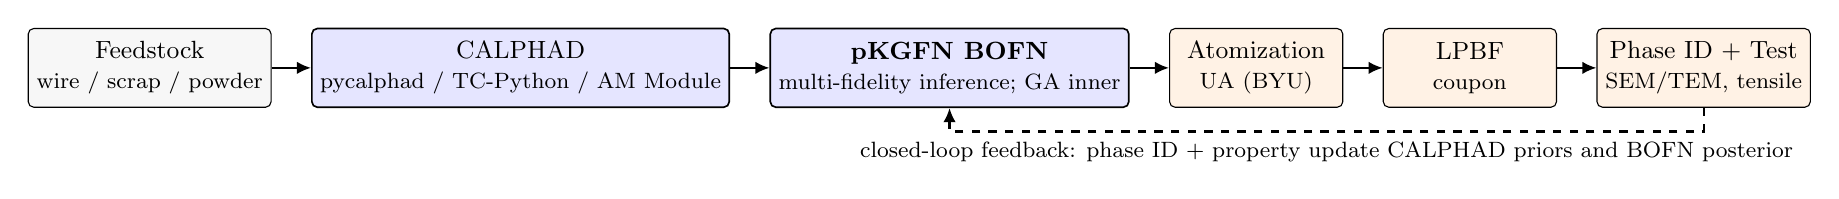
\begin{tikzpicture}[
    node distance=4.5mm and 5mm,
    every node/.style={font=\small},
    block/.style={rectangle, draw, rounded corners=2pt, align=center,
                  minimum height=10mm, minimum width=22mm, inner sep=3pt,
                  fill=black!3},
    ai/.style={block, fill=blue!10, line width=0.6pt},
    expt/.style={block, fill=orange!10},
    arr/.style={-{Latex[length=1.8mm,width=1.6mm]}, thick}
]
  \node[ai] (cal) {CALPHAD\\\footnotesize{pycalphad / TC-Python / AM~Module}};
  \node[ai, right=of cal] (bofn) {\bfseries pKGFN BOFN\\\footnotesize{multi-fidelity inference; GA inner}};
  \node[block, left=of cal] (feed) {Feedstock\\\footnotesize{wire / scrap / powder}};
  \node[expt, right=of bofn] (ua) {Atomization\\\footnotesize{UA (BYU)}};
  \node[expt, right=of ua] (lpbf) {LPBF\\\footnotesize{coupon}};
  \node[expt, right=of lpbf] (test) {Phase ID + Test\\\footnotesize{SEM/TEM, tensile}};
  \draw[arr] (feed) -- (cal);
  \draw[arr] (cal) -- (bofn);
  \draw[arr] (bofn) -- (ua);
  \draw[arr] (ua) -- (lpbf);
  \draw[arr] (lpbf) -- (test);
  % Loop-closure feedback arrow under the row.
  \draw[arr, dashed] (test.south) -- ++(0,-3mm) -| node[below, pos=0.25, font=\footnotesize]
      {closed-loop feedback: phase ID + property update CALPHAD priors and BOFN posterior} (bofn.south);
\end{tikzpicture}%
}
\end{center}


\section*{Problem}
Printable Al alloy families on the AMMTO trajectory rely on Co/Ni/Sc/REE additions; substitution toward domestically abundant Mn/Cr/Zr/Si/Fe streams requires a discovery loop that explicitly carries a feedstock supply-risk objective alongside printability and elevated-temperature strength. \textbf{Mapping to the 2023 DOE Critical Materials List:} the substitution targets directly displace Co (Critical 2025--2035), Sc/REE (Critical), and Ni (Near-Critical) by design --- each candidate alloy is evaluated against a per-element exposure score traceable to the current DOE list, scored by the CMI Hub. The Al--Ce trajectory (CMI Hub $\to$ Eck Industries $\to$ Magna) shows a CMI-coupled discovery$\to$validation pipeline can reach commercial deployment; no analogous trajectory yet exists for the Al--Mn--Cr--Zr / Al--Zr / Cu--Cr--Zr families that the FLAIME loop is positioned to address.

\section*{Idea, deliverable cadence, and go/no-go}
A 2--3~yr project applying the FLAIME discovery loop --- pKGFN BOFN over CALPHAD multi-fidelity nodes (\texttt{pycalphad}, TC-Python/TCAL10, AM~Module), validated by ultrasonic atomization (UA) and LPBF --- to one alloy family per project year. Baseline: Al--Mn--Cr--Zr and Al--Zr. Stretch (Y2--Y3): Cu--Cr--Zr or Be-substitution. \textbf{Hypothesis:} a supply-risk-aware BOFN--CALPHAD loop, with CMI-supplied feedstock data and Ames cross-check production runs, can deliver one TRL-4 candidate alloy and an associated UA feedstock specification per project year. \textbf{Annual go/no-go:} (i)~one validated candidate alloy with UA powder spec, LPBF parameter window, and tensile data at room and elevated temperature; (ii)~CMI-scored supply-risk reduction relative to the matched Al--Ce/Al--Ni--Sc benchmark; (iii)~Ames cross-check print confirming reproducibility outside BYU.

\section*{Cost-share and BABA compliance}
The 20\% statutory non-federal cost-share will be met by documented in-kind contributions from industrial partners, with BYU committing residual cost-share through PI summer salary and HPC; valuation, allowability, and PoP documentation will be audit-ready. \textbf{BABA:} the manufactured articles funded under this assistance are the UA-derived powder feedstock and the LPBF-produced Al alloy coupon/tested article; both are produced in the U.S. on the BYU-installed AMAZEMET rePOWDER and on U.S.-based LPBF systems. AMAZEMET's role is upstream engineering support (process know-how transfer), not procurement of foreign-manufactured end product; no foreign-manufactured iron, steel, or manufactured product is incorporated into the deliverable article stream. If contracting determines a waiver is needed, Valimet provides a fully domestic atomization comparator path. Any EU mirror-site engineering interaction is knowledge exchange only and will be disclosed under research-security review.

\section*{Partnership structure and downstream-adopter pathway}
\textbf{Funded:} BYU (Baird, lead --- discovery loop, in-house UA powder synthesis, LPBF coordination); CMI Hub (supply-chain modeling, supply-risk scoring, reference validation prints under separate CMI funding). \textbf{Collaborator with own funding:} Ames Laboratory (cross-check production runs; per AMMTO/EERE convention Ames brings its own DOE funding rather than a budget line through BYU). \textbf{Industrial:} Valimet, AMAZEMET, Thermo-Calc (CALPHAD). \textbf{Downstream adopter (gap acknowledged, in-progress):} no Eck/Magna-class transition partner is yet under letter for Al-MPEA; before the full white paper we will close one of two paths --- LPBF service bureau adopting the qualified powder/parameter window, or automotive/aerospace tier-1 evaluator analogous to Magna's Al-Ce role --- and disclose the named partner.

\section*{Preliminary results (FLAIME pipeline, BYU, Apr~2026)}
UA composition modification from AlSi10Mg + Al wire + Si feed confirmed by SEM/EDS; Thermo-Calc AM~Module simulations on candidate FLAIME compositions; CALPHAD jobs on BYU HPC. AlSi10Mg LPBF tensile baseline; elevated-temperature tensile data on a standard Al specimen; working pKGFN BOFN; automated powder dispensing demonstrated. The Ames letter of support is on file. \emph{Y1 risk-retiring milestone:} one Al-Mn-Cr-Zr or Al-Zr LPBF coupon set produced via the proposed feedstock route, with printability evidence, room-temperature tensile vs.~AlSi10Mg, and a per-element exposure-score delta vs.~an Sc/REE-bearing comparator --- the closed-loop result reviewers will want before TRL-4 claims.

\section*{Scope separation from pending DOE Genesis Mission Topic~3B and request}
\textbf{Task-level scope separation.} \emph{Genesis tasks (DOE / Topic~3B):} alloy-agnostic platform construction --- hardware integration, scheduler, data fabric, autonomous orchestration, general platform validation. \emph{AMMTO tasks (this proposal):} (T1)~per-alloy-family campaign design with explicit critical-materials-list mapping; (T2)~UA powder production and qualification; (T3)~LPBF parameter-window development; (T4)~elevated-temperature mechanical testing to TRL-4; (T5)~CMI-scored supply-risk benchmarking and Ames cross-check. Personnel labor is itemized per task; data packages and reporting artifacts are alloy-family-specific and not Genesis-platform deliverables. No budget line, equipment purchase, or scheduler/data-fabric task appears in both. \textbf{Request:} a scoping call with the cognizant AMMTO PM and the CMI Hub director (via the Ames letter contact) to confirm the per-element exposure score and TRL-4 framing match the current Critical Materials List before we draft a full white paper.

{\footnotesize \emph{Repo:} \url{https://github.com/vertical-cloud-lab}.}

\end{document}
